\documentclass[11pt]{article}
\usepackage{fullpage,amsthm,amsfonts,amssymb,epsfig,amsmath,times,amsthm}
\usepackage{algpseudocode}
\usepackage{tikz}
\usepackage{ulem}
\usepackage{listings}
\usepackage{color}
\usepackage{unicode-math}

\def\checkmark{\tikz\fill[scale=0.4](0,.35) -- (.25,0) -- (1,.7) -- (.25,.15) -- cycle;}

\definecolor{dkgreen}{rgb}{0,0.6,0}
\definecolor{gray}{rgb}{0.5,0.5,0.5}
\definecolor{mauve}{rgb}{0.58,0,0.82}

\newtheorem{theorem}{Theorem}
\newtheorem{claim}[theorem]{Claim}
\newtheorem*{solution}{Solution}


\usepackage{cse103}
\def\title{HW 1}
\begin{document}
\maketitle

\section*{Due October 6 at 11:59pm}

\textbf{(5 questions, 215 points total)}

\begin{qunlist}
  \q{25}{Alphabets and Strings}\\
  Let $\Sigma = \{ a, b, c \}$.
  Recall that we denote the empty string by $\epsilon$.
  \begin{qparts}
    \item
    What is the set $\Sigma^2$?
    \begin{solution}
      \begin{equation}
        \Sigma^2 = \{aa,ab,ac,ba,bb,bc,ca,cb,cc \}
      \end{equation}
    \end{solution}

    \item
    What is $|\Sigma^5|$?
    \begin{solution}
      \begin{equation}
        |\Sigma^5| = 3^5 = 243
      \end{equation}
    \end{solution}

    \item
    What is the set $\{ w_4 w_6 \st w \in \Sigma^{8} \}$?
    \begin{solution}
      Due to the nature of sets containing only unique elements and the above set constructor is a set of elements with only length 2 therefore the set constructor is equivalent to $\Sigma^2$.
      \begin{equation}
        \{ w_4 w_6 \st w \in \Sigma^{8} \} \equiv \Sigma^2 = \{aa,ab,ac,ba,bb,bc,ca,cb,cc \}
      \end{equation}
    \end{solution}

    \item
    What is the set $\{ w \in \Sigma^* \st |w| = 0 \text{ or } |w| = 1 \}$?
    \begin{solution}
      \begin{equation}
        \{ w \in \Sigma^* \st |w| = 0 \text{ or } |w| = 1 \} = \{\epsilon,a,b,c\}
      \end{equation}
    \end{solution}

    \item
    What is the set $\{ xx \st x \in \Sigma \}$?
    \begin{solution}
      \begin{equation}
        \{ xx \st x \in \Sigma \} = \{aa,bb,cc\}
      \end{equation}
    \end{solution}

  \end{qparts}

  \newpage

  \q{30}{Languages}\\
  Let $\Sigma = \{0, 1\}$.
  For each of the following pairs of languages over $\Sigma$, state whether they are equal ($=$), one is a proper subset of the other ($\subset$), or if they are incomparable (neither is a subset of the other).
  If $L_1 \subset L_2$, give an example of a string in $L_2$ that is not in $L_1$, or vice versa if $L_2 \subset L_1$; if the languages are incomparable, give an example string from each language that is not in the other.
  \begin{qparts}
    \item
    $L_1 = \Sigma^2 \cup \Sigma^4$ \\
    $L_2 = \Sigma^{6}$
    \begin{solution}
      $L_1$ and $L_2$ are incomparable:
      \begin{gather}
        L_1 = 01 or 0110\\
        L_2 = 0110110
      \end{gather}
      $|L_1|$ will always be either 2 or 4 and $|L_2|$ will always be 6 therefore $L_1$ and $L_2$ are incomparable.
    \end{solution}

    \item
    $L_1 = \{1\}^*$ \\
    $L_2 = \{ x \in \Sigma^* \st |x| \text{ is odd} \}$
    \begin{solution}
      $L_1$ and $L_2$ are incomparable:
      \begin{gather}
        L_1 \neq L_2\\
        L_1 = 11 \not\subset L_2\\
        L_2 = 101 \not\subset L_1
      \end{gather}
      $L_1$ and $L_2$ are incomparable because there are aspects of each language that are not present in the other even there is some overlap.
    \end{solution}

    \item
    $L_1 = \{ x \in \Sigma^8 \st \exists y \in \Sigma^* . \; x = yyy \}$ \\
    $L_2 = \Sigma^3 \cap \Sigma^8$ \\
    \quad (N.B. The dot in $L_1$ simply indicates the end of the quantifier $\exists y \in \Sigma^*$; you can read the condition as ``there exists some $y \in \Sigma^*$ such that $x = yyy$''.)
    \begin{solution}
      $L_1$ and $L_2$ are equal:
      \begin{gather}
        L_1 = L_2\\
        L_1 = \emptyset \\
        L_2 = \emptyset
      \end{gather}
      $L_1$ and $L_2$ are equal because within $L_1$ there is no $y$ when concatenated 3 times ($x=yyy$) will equal to an $x$ that is 8 digits long. $\frac83$ is not an integer that can match a $y$. Therefore $L_1$ is null/empty. Similarly there is no intersect (common elements) between $\Sigma^3$ and $\Sigma^8$ which results in again a null/empty set thereby resulting in $L_1$ and $L_2$ being equal.
    \end{solution}

    \item
    $L_1 = \Sigma^*$ \\
    $L_2 = \cup_{k \ge 1} \Sigma^k$
    \begin{solution}
      \begin{gather}
        L_2 \subset L_1\\
        L_1 = \Sigma^{\star}\\
        L_2 = \cup_{k \ge 1} \Sigma^k = \Sigma^{1} + \Sigma^{1} + \cdots \Sigma^{\infty} \\
        \nonumber L_2 = \Sigma^{\star}-\epsilon\\
        L_1 = \epsilon \not\in L_2
      \end{gather}
      $L_2$ is a subset of $L_1$ because $\Sigma^0$ is $\epsilon$ and $L_2$ excludes $\Sigma^0$.
    \end{solution}

    \item
    $L_1 = \{ x \in \Sigma^* \st x \text{ is a binary encoding of a prime number} \}$ \\
    $L_2 = \{ 10 \} \cup \{ x \in \Sigma^* \st \text{the last symbol of $x$ is 1} \}$
    \begin{solution}
      $L_1$ is a subset of $L_2$:
      \begin{gather}
        L_1 \subset L_2\\
        L_1 = 101 \subset L_2\\
        L_2 = 1001 \not\subset L_1
      \end{gather}
      $L_1$ is a subset of $L_2$ because $L_1$ encodes prime numbers which can be odd or even but $L_2$ encodes the number $2$ and every odd number that follows and $1001$ is equal to $9$ which is not a prime number.
    \end{solution}

  \end{qparts}

  \newpage

  \q{50}{Working with a DFA}\\
  Consider the DFA $M = (Q, \Sigma, \delta, q_0, F)$ where:
  \begin{itemize}
    \item $Q = \{ 1, 2, 3, 4 \}$
    \item $\Sigma = \{ a, b \}$
    \item $\delta(q, s) =
            \begin{cases}
              1 \quad q = 2 \text{ or } s = b  \\
              3 \quad q = 1 \text{ and } s = a \\
              4 \quad \text{otherwise}
            \end{cases}$
    \item $q_0 = 2$
    \item $F = \{ 1, 4 \}$
  \end{itemize}

  \begin{qparts}
    \item \emph{(20 pts.)}
    Draw $M$ as a graph.
    \begin{solution}
    \end{solution}
    \begin{align}
      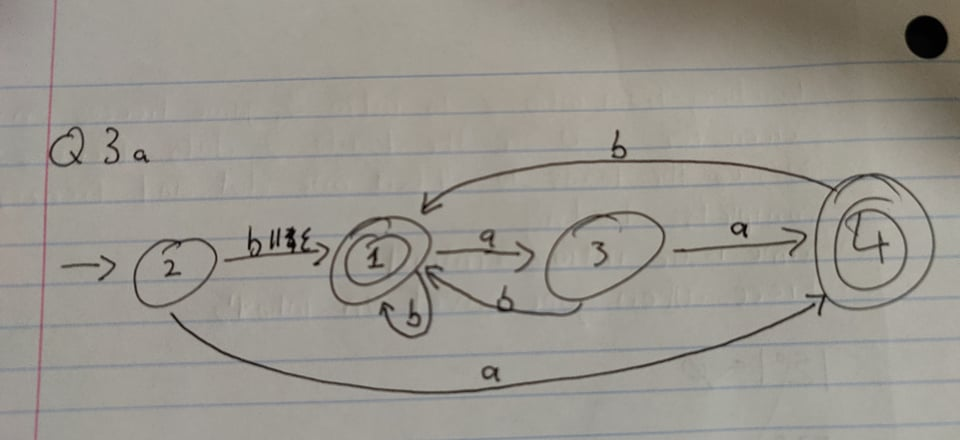
\includegraphics[width=5in]{3a}
    \end{align}

    \item \emph{(18 pts.)}
    Which of the following strings does $M$ accept: $\epsilon, b, a, ba, aaa, baab$?
    Give an accepting path (the sequence of states traced out by the DFA as it executes) for each accepted string.

    \begin{solution}
      Format: \newline $\mbox{input } \Rightarrow \mbox{ list of inputs over states separated by $\rightarrow$ with the last state being the end then $\checkmark$ or $\times$ } $
      \begin{gather}
        \epsilon \Rightarrow \frac{\epsilon}2 \rightarrow 1 \hspace{20pt} \checkmark\\
        b \Rightarrow \frac b 2 \rightarrow 1 \hspace{20pt} \checkmark\\
        a \Rightarrow \frac a 2 \rightarrow 4 \hspace{20pt} \checkmark\\
        ba \Rightarrow \frac b 2 \rightarrow \frac a 1 \rightarrow 3 \hspace{20pt} \times\\
        aaa \Rightarrow \frac a 2 \rightarrow \frac a 4\rightarrow \frac a 4\rightarrow 4 \hspace{20pt} \checkmark\\
        baab \Rightarrow \frac b 2 \rightarrow \frac a 1\rightarrow \frac a 3\rightarrow \frac b 4 \rightarrow 1 \hspace{20pt} \checkmark\\
      \end{gather}
    \end{solution}

    \item \emph{(12 pts.)}
    What is the language $L(M)$ of $M$?
    \begin{solution}
      $L(M) = $ all strings over $\Sigma = \{a,b\}$ that don't end with substring "ba".
    \end{solution}
  \end{qparts}

  \newpage

  \q{60}{Designing DFAs}\\
  For each of the following languages, draw a DFA (as a graph) recognizing it:
  \begin{qparts}
    \item
    All strings over $\Sigma = \{a, b, c\}$ which either contain an $b$ or contain \emph{both} an $a$ and a $c$.
    \begin{solution}
    \end{solution}
    \begin{align}
      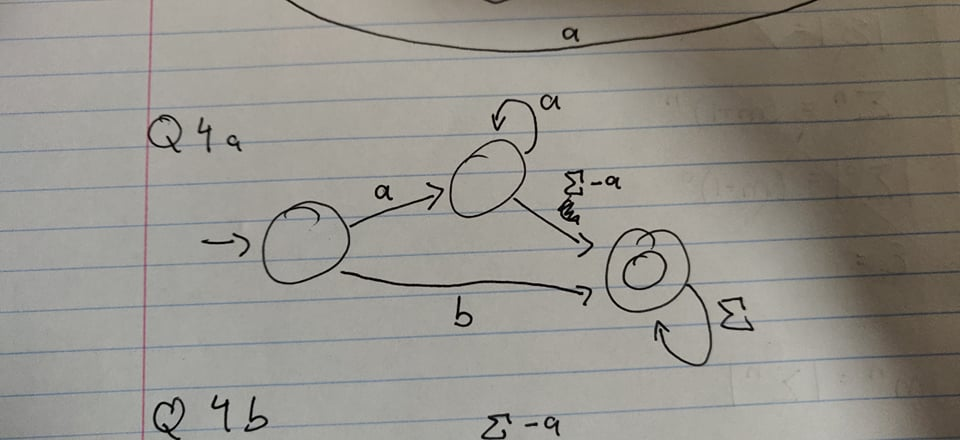
\includegraphics[width=5in]{4a}
    \end{align}

    \item
    All strings over $\Sigma = \{a, b, c, \dots, z\}$ containing the substring $aaa$.
    \begin{solution}
    \end{solution}
    \begin{align}
      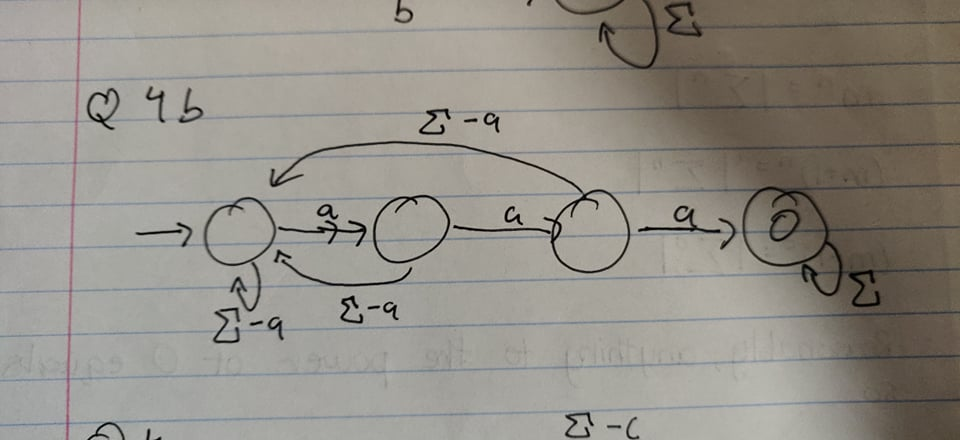
\includegraphics[width=5in]{4b}
    \end{align}
    \newpage
    \item
    All strings over $\Sigma = \{a, b, c\}$ which are in alphabetical order (e.g. $aaac$ and $bcc$ but not $aba$ or $ca$).
    \begin{solution}
    \end{solution}
    \begin{align}
      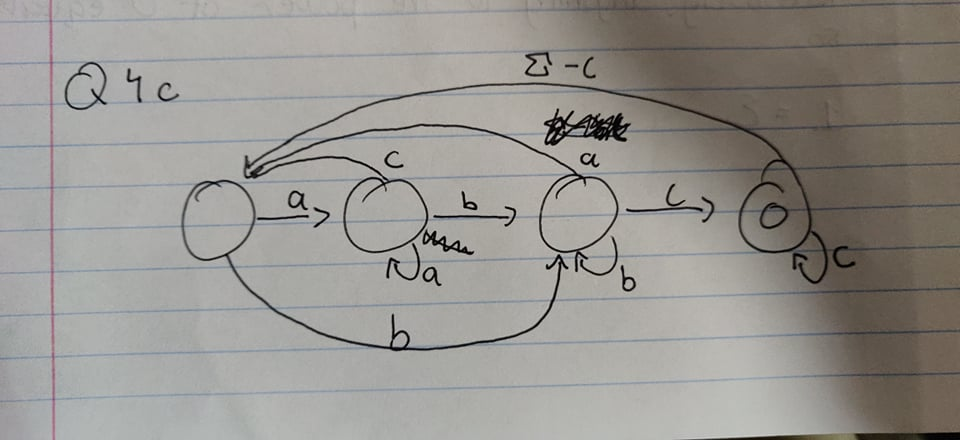
\includegraphics[width=5in]{4c}
    \end{align}

  \end{qparts}

  \newpage

  \q{50}{Counting Strings}\\
  We argued in class that given an alphabet $\Sigma$ with $m = |\Sigma|$ symbols, there are $m^n$ strings of length $n$: $|\Sigma^n| = m^n$.
  Let's prove this formally for any $m \ge 1$ and $n \ge 0$ using induction.
  \begin{qparts}
    \item
    Which quantity should we do the induction on?
    \begin{solution}
      Let us begin induction on variable $n$.
    \end{solution}

    \item
    Choose a base case and state the claim you need to prove for it.
    \begin{solution}
      Base case: $n=0$
    \end{solution}

    \item
    Prove the base case.
    \begin{solution}
      \begin{gather}
        |\Sigma^n| = m^n\\
        |\Sigma^0| = \left(m\right)^0\\
        |\Sigma^0| = |\epsilon| = 1= \left(m\right)^0
      \end{gather}
    \end{solution}

    \item
    State the claim you need to prove for the inductive case, and the inductive hypothesis you can assume while proving it.
    \begin{solution}
      \begin{align}
        \mbox{Claim: }|\Sigma^{n+1}| = \left(m\right)^{n+1} \\
        \mbox{Hypothesis: }|\Sigma^n| = \left(m\right)^n
      \end{align}

    \end{solution}

    \item
    Prove the inductive case.
    \begin{solution}
      \begin{gather}
        |\Sigma^{n+1}| = \left(m\right)^{n+1}\\
        |\Sigma^{n+1}| = \left(m\right)^n \cdot m\\
        |\Sigma^{n+1}| = |\Sigma^n| \cdot m\\
        \frac{|\Sigma^{n+1}|}{|\Sigma^n|} = m\\
        \left|\frac{\Sigma^{n+1}}{\Sigma^n}\right| = m\\
        |\Sigma^n| = m
      \end{gather}
    \end{solution}

    \item
    Conclude your proof of the original statement.
    \begin{solution}
      Due to $|\Sigma^n| = \left(m+1\right)^n$ holding true when $n =(n+1)$ then for any $n \geq 0$ the aforementioned statement must also hold true thereby $|\Sigma^n| = \left(m\right)^n$ should also hold true
    \end{solution}
  \end{qparts}

  N.B. Whenever doing a proof by induction, make sure to include all of the information above. You don't have to break up your presentation into as many pieces as we did here, but you need to clearly state what you're proving by induction, separate the base and inductive cases, etc. For example, I often use language like ``We prove this for all $k \in \{0, \dots, n\}$ by induction on $k$ in decreasing order. In the base case $k = n$, we have...'', and then in a new paragraph for the inductive case, ``Now suppose the hypothesis holds for $k > 0$; then it also holds for $k-1$ because...''.

\end{qunlist}
\end{document}